\documentclass{article}

\usepackage{styles/arxiv}

\usepackage[utf8]{inputenc} % allow utf-8 input
\usepackage[T1]{fontenc}    % use 8-bit T1 fonts
\usepackage{hyperref}       % hyperlinks
\usepackage{url}            % simple URL typesetting
\usepackage{booktabs}       % professional-quality tables
\usepackage[english]{babel}
\usepackage{nicefrac}       % compact symbols for 1/2, etc.
\usepackage{microtype}      % microtypography
\usepackage{graphicx}
\usepackage{stmaryrd}

\usepackage{amsthm}
\usepackage{amssymb}
\usepackage{amsfonts}
\usepackage{amsmath}
\usepackage{mathtools}

\usepackage{tikz}
\usepackage{qtree}

\usepackage{listings}
\lstset{
  basicstyle=\itshape,
  xleftmargin=3em,
  literate={->}{$\rightarrow$}{2}
           {α}{$\alpha$}{1}
           {δ}{$\delta$}{1}
}

\usepackage{xstring}
\usepackage{stmaryrd}
\usepackage{wasysym}
\usepackage{textcomp}
\usepackage{blindtext}
\usepackage{subfiles}

\newtheorem{definition}{Definition}
\numberwithin{definition}{section}
\newtheorem{lemma}{Lemma}
\numberwithin{lemma}{section}
\newtheorem{proposition}{Proposition}
\numberwithin{proposition}{section}
\newtheorem{corollary}{Corollary}
\numberwithin{corollary}{section}
\newtheorem{theorem}{Theorem}
\numberwithin{theorem}{section}

\DeclareMathSymbol{\mathinvertedexclamationmark}{\mathclose}{operators}{'074}
\DeclareMathSymbol{\mathexclamationmark}{\mathclose}{operators}{'041}
\makeatletter
\newcommand{\raisedmathinvertedexclamationmark}{%
  \mathclose{\mathpalette\raised@mathinvertedexclamationmark\relax}%
}
\newcommand{\raised@mathinvertedexclamationmark}[2]{%
  \raisebox{\depth}{$\m@th#1\mathinvertedexclamationmark$}%
}
\begingroup\lccode`~=`! \lowercase{\endgroup
  \def~}{\@ifnextchar`{\raisedmathinvertedexclamationmark\@gobble}{\mathexclamationmark}}
\mathcode`!="8000
\makeatother

\newcommand{\intga}{\mathclap{\smash{\oplus}}{\int}}
\newcommand{\intgp}{\mathclap{\smash{\otimes}}{\int}}
\newcommand{\intgg}{\mathclap{\rightsquigarrow}\mathclap{\int}}

\title{Geometry of Arithmetic Expressions: I.\\ Basic Concepts and Unsolved Problems}

%\date{Decmber 8, 2022}	% Here you can change the date presented in the paper title
%\date{} 				% Or removing it

\author{
  Mingli~Yuan \\
  AI Lab \\
  ColorfulClouds Tech.\\
  Beijing, 100083 \\
  \texttt{mingli.yuan@gmail.com}
}

% Uncomment to remove the date
%\date{}

% Uncomment to override  the `A preprint' in the header
\renewcommand{\headeright}{A preprint}
\renewcommand{\undertitle}{A preprint}

\begin{document}
\maketitle

\begin{abstract}
    TODO
\end{abstract}

\keywords{arithmetic expressions, hyperbolic geometry}

\setcounter{tocdepth}{2}
\tableofcontents
\newpage

\section{Introduction}\label{sec:introduction}

Can arithmetic expressions form a geometric space?
In this paper, we present several examples of arithmetic expression spaces and examine their properties.

TODO

\subsection{Arithmetic expression}

In order to define arithmetic expressions involving real numbers  $\mathbb{R}$ in a rigorous way, we need to use a sophisticated type theory.
However, in order to keep things simple and maintain clarity, we will start by using only production rules,
but with certain semantic restrictions. We will also begin with rational numbers $\mathbb{Q}$ to avoid the difficulties inside real numbers $\mathbb{R}$ .

\begin{definition}\label{def:arithmetic-expression}
    An arithmetic expression $a$ over $\mathbb{Q}$ is a structure given by the following production rules:
\begin{equation}\label{eq:productionrule}
\begin{aligned}
a &\longleftarrow x\\
a &\longleftarrow ( a + a )\\
a &\longleftarrow ( a - a )\\
a &\longleftarrow ( a \times a )\\
a &\longleftarrow ( a + a )
\end{aligned}
\end{equation}
    where $x \in \mathbb{Q}$, and we denote this as $a \in \mathbb{E} \left [\mathbb{Q} \right ]$.

\end{definition}

During the production process, we can obtain both a string representation and a tree representation of arithmetic expression $a$,
where the two representations are equivalent. For instance, the string representation of $a$ might be:

\begin{equation}
(((((1 \times 2) \times 2) - 1) \times (2 + 1)) - 6)
\end{equation}

and the parsed syntax tree is depicted in Figure \ref{fig:syntaxtree}.

\begin{figure}[ht]
\centering
\resizebox{0.2\textheight}{!}{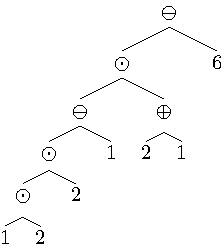
\includegraphics{images/02-example-expression-syntax-tree.pdf}}
\caption{a tree representation of an arithmetic expression}\label{fig:syntaxtree}
\end{figure}

If we interpret the target as a string and the building processes in production rule \eqref{eq:productionrule} as string building,
we get the \emph{string representation}. On the other hand, if the target is a tree, tree building leads to the \emph{tree representation}.
We can easily obtain the string representation of $a$ from its tree representation by performing a pre-order traversal.

The concept of a \emph{sub-expression} can also be derived from the concept of a sub-tree.
The branch nodes are all labeled with operators: $+$, $-$, $\times$, $\div$. The leaf nodes are all labeled with numbers.

Evaluation $\nu$ is a partial function that operates on arithmetic expression $a \in \mathbb{E} \left [\mathbb{Q} \right ]$.
It is undefined only if division by zero occurs during the recursive evaluation process.

We can define evaluation $\nu(a)$ of $a$ recursively as follows:
\begin{itemize}
  \item Constant leaf: for any $x \in \mathbb{Q}$, $\nu(x) = x$.
  \item Compositional node by $+$: For any $(a + b)$, $\nu((a + b)) = \nu(a) + \nu(b)$.
  \item Compositional node by $-$: For any $(a - b)$, $\nu((a - b)) = \nu(a) - \nu(b)$.
  \item Compositional node by $\times$: For any $(a \times b)$, $\nu((a \times b)) = \nu(a) \nu(b)$.
  \item Compositional node by $\div$: For any $(a \div b)$, if $\nu(b) \neq 0$, then $\nu((a \div b)) = \nu(a) / \nu(b)$.
\end{itemize}

We say that an arithmetic expression $a$ is \emph{evaluable} if $\nu(a)$ is defined.
In the rest of this article, we will only consider evaluable arithmetic expressions unless stated otherwise.

Given an arithmetic expression $a$, whatever evaluable or not, we can obtain its tree representation.
If a node $l$ is a leaf node, its corresponding subexpression $s$ is a number, so we consider it to be already "evaluated".
If a node $b$ is a branch node, its corresponding subexpression $s$ is an expression, and we can apply $\nu$ to it to obtain a number $\nu(s)$.
During the recursive evaluation process, starting from the leaves and moving towards the root, the subexpressions are evaluated one after another.
However, the order of evaluations is generally not unique.

\begin{definition}
The evaluation order of an arithmetic expression $a$ is an ordering of branch nodes in the tree representation of $a$
such that every node (sub-expression) is evaluated before its parent.
\end{definition}

For example, the possible evaluation orders of the arithmetic expression in Figure \ref{fig:syntaxtree} are:
\begin{itemize}
  \item $1 \times 2 \rightarrow 2; 2 \times 2 \rightarrow 4; 4 - 1 \rightarrow 3; 2 + 1 \rightarrow 3; 3 \times 3 \rightarrow 9; 9 - 6 \rightarrow 3$
  \item $1 \times 2 \times 2 - (2 + 1) \times 1 - 6$
\end{itemize}

Below are examples of expressions that have a unique evaluation order. These include right-expanded, left-expanded,
and combinations of them, as shown in Figure \ref{fig:leftright} and Figure \ref{fig:combination}.

\begin{figure}[ht]
\centering
\resizebox{0.4\textheight}{!}{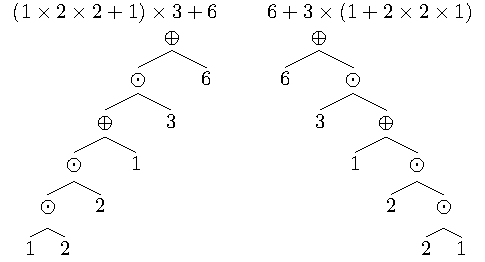
\includegraphics{images/03-example-expression-syntax-tree-left-right.pdf}}
\caption{right-expanded and left-expanded expressions}\label{fig:leftright}
\end{figure}

\begin{figure}[ht]
\centering
\resizebox{0.2\textheight}{!}{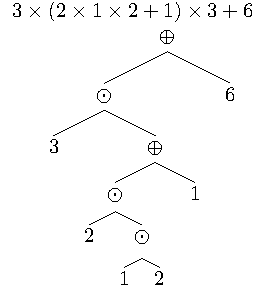
\includegraphics{images/04-example-expression-syntax-tree-combination}}
\caption{combinations of right-expanded and left-expanded expressions}\label{fig:combination}
\end{figure}

\begin{definition}
A threadlike expression is an arithmetic expression that all the left nodes in its tree representation are leaf nodes.
\end{definition}

So a threadlike expression is right-expanded and its evaluation order is unique.

Threadlike expressions are significant because they are analogous to the concept of paths in homotopy theory in geometry.

\subsection{A scalar field and a mesh grid}\label{sec:meshgrid}

Consider the upper half plane $\{\mathcal{H}: (x, y) | y > 0 \}$ equipped with an inner product and metrics defined as follows:

$$
\mathbf{a} \cdot \mathbf{b} = \begin{bmatrix} a_x & a_y \end{bmatrix} \begin{bmatrix} \frac{1}{y^2} & 0 \\ 0 & \frac{1}{y^2 \ln^2 2} \end{bmatrix} \begin{bmatrix} b_x \\ b_y \end{bmatrix}
$$

and

$$
ds^2 = \frac{1}{y^2} (dx^2 + \frac{dy^2}{\ln^2 2})
$$

We consider a scalar field satisfying

\begin{equation}
A = - \frac{x}{y}
\end{equation}

We call this field an \emph{assignment}.

Proper assignments allow us to establish a connection between paths in homotopy and threadlike arithmetic expressions,
and to incorporate function theory into the study of arithmetic expression geometry.

\begin{figure}[ht]
\centering
\resizebox{0.9\textwidth}{!}{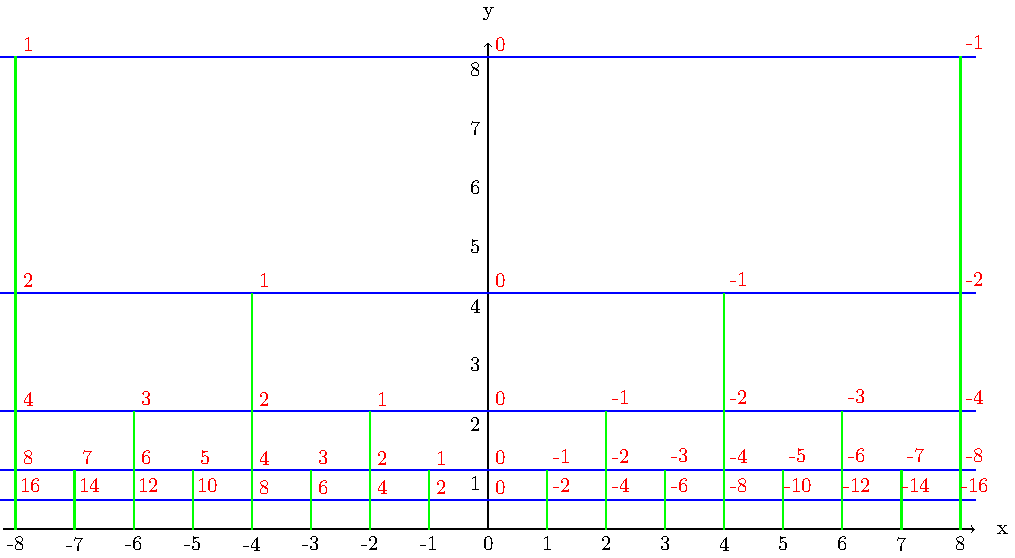
\includegraphics{images/01-grid-example-1.pdf}}
\caption{An addition-multiplication grid by generators with $\mu=1$ and $\lambda=\ln 2$}\label{fig:gridex0}
\end{figure}

We can draw a grid on the scalar field $A$ and underlying upper half plane $\mathcal{H}$ as shown in Figure \ref{fig:gridex0}.
The blue lines encode a $+ 1$ relationship, the green lines encode a $\times 2$ relationship,
and they are line families that are perpendicular to each other.
The length of the line segments between two neighboring crossing points are unit length(calculations in lemma \ref{lem:regular}).
The red value at the crossing points is the value of the scalar field $A$ at that point.
Based on the relationships encoded by the lines, we can encode threadlike arithmetic expressions,
which will be introduced in the subsection \ref{sec:encoding}.

The addition-multiplication grid is also scale-invariant under the transformation
$$
\begin{cases}
x' = \alpha x\\
y' = \alpha y
\end{cases}
$$

where $\alpha = 2^k , k \in \mathbb{Z}$.

We can image if we make the grid finer and finer, the grid will become a continuous space.
This leads to a rigorous treatment of arithmetic expressions as a geometric space in section \ref{sec:topology}.

\subsection{Encoding threadlike expressions on the addition-multiplication gird}\label{sec:encoding}

If we interpret the horizontal blue lines as $+ 1$ and the vertical green lines as $\times 2$ in Figure \ref{fig:gridex0},
we can encode threadlike expressions on the addition-multiplication grid. For example, in Figure \ref{fig:encoding}
we encode $((((1 \times 4) - 1) \times 2) - 3)$ as the bold black lines.

\begin{figure}[ht]
\centering
\resizebox{0.9\textwidth}{!}{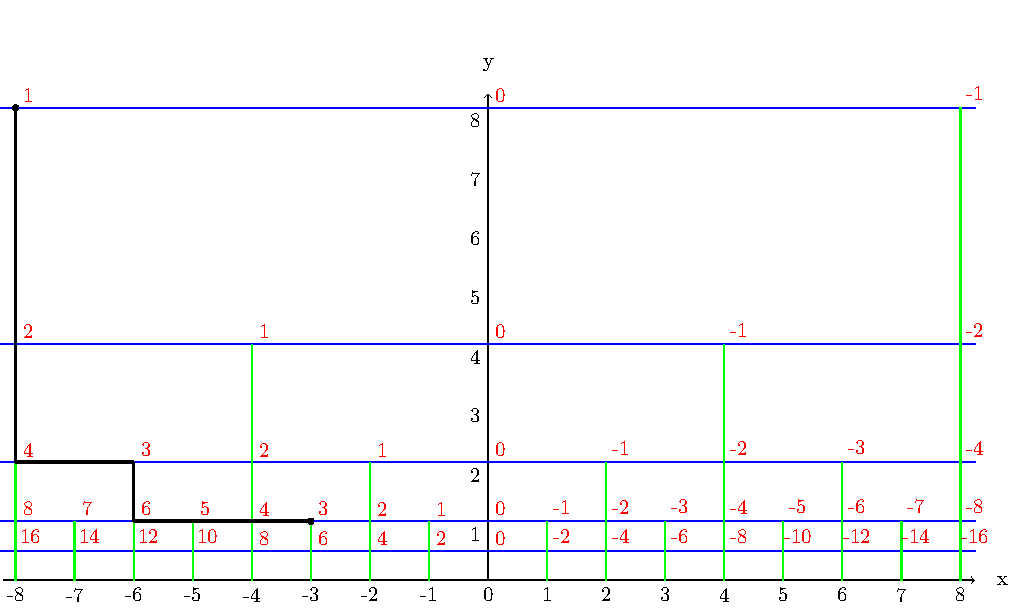
\includegraphics{images/05-example-expression-embedding}}
\caption{encoding threadlike expression}\label{fig:encoding}
\end{figure}

The zigzag lines in Figure \ref{fig:encoding} can be divided into four parts:
\begin{itemize}
\item the vertical line from $1$ to $4$: encoded as multiplication by $4$
\item the horizontal line from $4$ to $3$: encoded as subtraction by $1$
\item the vertical line from $3$ to $6$: encoded as multiplication by $2$
\item the horizontal line from $6$ to $3$: encoded as subtraction by $3$
\end{itemize}

\subsection{From a scalar field to a space of threadlike expressions}

As shown in Figure \ref{fig:canonicalform}, we have the following paths and expressions:
\begin{itemize}
\item the black path: $((1 \times 8) - 5) = 3$
\item the purple path: $((1 - \frac{5}{8}) \times 8) = 3$
\item the brown path: $((((((1 - \frac{1}{8}) \times 2) - \frac{1}{2}) \times 2) - 1) \times 2) = 3$
\item the orange path: infinit many addition-multiplication terms accumulated together, a special kind of integration
\end{itemize}

\begin{figure}[ht]
\centering
\resizebox{0.9\textwidth}{!}{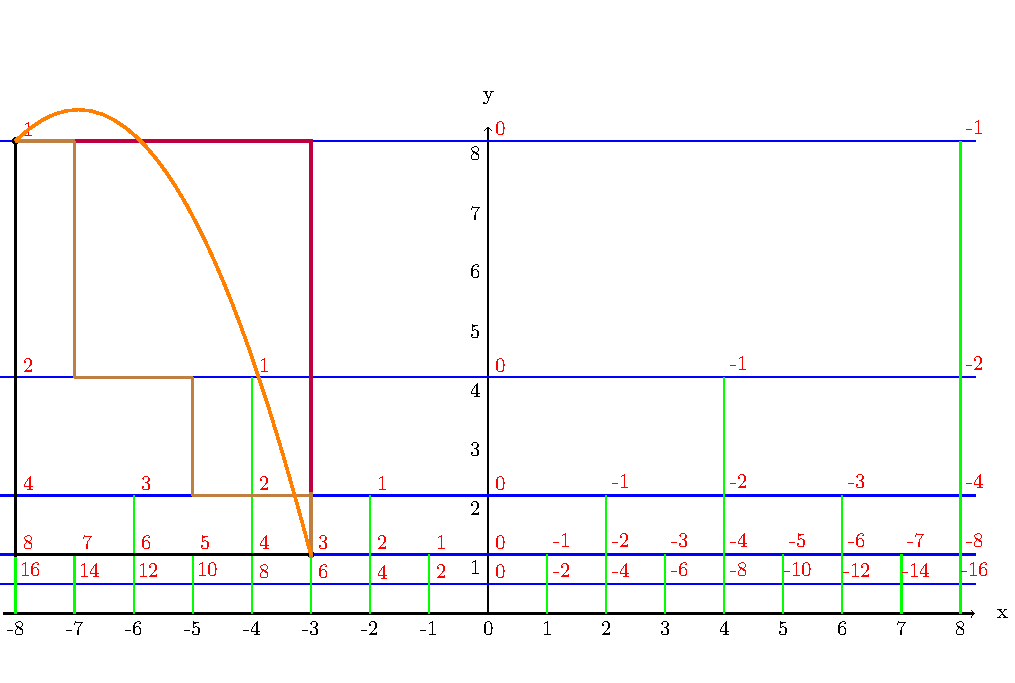
\includegraphics{images/06-example-canonical-form}}
\caption{different encodings and their canonical form}\label{fig:canonicalform}
\end{figure}

All of the paths in Figure \ref{fig:canonicalform} have the same source $1$ and same target $3$. We will discuss a canonical form for these paths.

It is easy to see that the expressions can be transformed into each other by using the multiplication distributive law and by combining and decomposing terms.

Conversion form brown path to black path
\begin{align}
3 & = ((((((1 - \frac{1}{8}) \times 2) - \frac{1}{2}) \times 2) - 1) \times 2) \\
& = 1 \times 8 -  \frac{1}{8} \times 8 - \frac{1}{2} \times 4 - 1 \times 2 \\
& = ((1 \times 8) - 5)
\end{align}

Conversion form brown path to purple path
\begin{align}
3 & = ((((((1 - \frac{1}{8}) \times 2) - \frac{1}{2}) \times 2) - 1) \times 2) \\
& = (1 - \frac{1}{8}) \times 8 - \frac{1}{2} \times 4 - 1 \times 2 \\
& = (1 - \frac{1}{8}) \times 8 - \frac{1}{4} \times 8 -  \frac{1}{4} \times 8 \\
& = (1 - \frac{1}{8} - \frac{1}{4} - \frac{1}{4}) \times 8 \\
& = ((1 - \frac{5}{8}) \times 8)
\end{align}

Therefore, we can define the black and purple paths in Figure \ref{fig:canonicalform} as a pair of canonical paths,
which represent all threadlike expressions connecting the source $1$ and the target $3$.

Once we have such canonical paths, we can determine the canonical form of the whole space relative to an arbitrary source point $O$
and any other target point $P$. This allows us to define the space as a space of threadlike expressions.

\subsection{Currying and path notation}

Currying is a basic technique in functional programming, which is used to transform a function with multiple arguments into a sequence of functions with one argument.
By currying a threadlike arithmetic expression, we can obtain a sequence of functions that operate on an operand, which is the leftmost leaf node.

We introduce the following notation for currying a threadlike arithmetic expression:
\begin{itemize}
    \item initial operand: the leftmost leaf node
    \item operator: $\oplus_y: x \mapsto x + y$
    \item operator: $\ominus_y: x \mapsto x - y$
    \item operator: $\otimes_y: x \mapsto x \cdot e^y$
    \item operator: $\oslash_y: x \mapsto x \cdot e^{-y}$
\end{itemize}

For example, the threadlike arithmetic expression $(((((1 \times 2) \times 2) + 1) \times 3) + 6)$ can be curried as

$$\oplus_6(\otimes_{\ln 3}(\oplus_1(\otimes_{\ln 2}(\otimes_{\ln 2}(1)))))$$

Suppose we have a series of operators $a_1, a_2, \cdots a_{n-1}, a_n$, we introduce a \emph{path notation}.

$$x a_1 a_2 \cdots a_{n-1} a_n \coloneqq a_n( a_{n-1}( \cdots a_2( a_1(x) ) \cdots ) )$$

So, the above example can be written as

$$1 \otimes_{\ln 2} \otimes_{\ln 2} \oplus_1 \otimes_{\ln 3} \oplus_6 $$

If a path begins with a number, we refer to it as a \emph{bounded path}.
If it does not, we refer to it as a \emph{free path}, similar to the concept of vectors from the origin versus vectors at arbitrary points.
a bounded path results in a number, while a free path results in a function.

Now we will verify that the operators within a path are associative.

\begin{lemma}\label{lemma:associative}
    The operators within a path are associative, i.e. we have $$a (b c) = (a b) c$$
\end{lemma}

\begin{proof}
For a free path, follow the definition, we have
$$a (b c) = (b c)(a) = c(b(a))$$
$$(a b) c = c (a b) = c(b(a))$$

For a bounded path, we have
$$x a (b c) = (b c)(a(x)) = c(b(a(x)))$$
$$x (a b) c = c((a b)(x)) = c(b(a(x)))$$
\end{proof}

\begin{definition}\label{definition:concatenate}
    The concatenation of paths $p_1 \cdot p_2$ is defined as the composite of functions:
    $$p_1 \cdot p_2 \coloneqq p_2 \circ p_1 $$
\end{definition}

When a sequence of paths is concatenated, and only the first path can be bounded.
If the first path is bounded, the concatenated result is a bounded path.
Otherwise, the concatenated result is a free path.

\subsection{Generated structure and problems on equality, sigularity, symmetries}

In order to study mesh grids like the one described in subsection \ref{sec:meshgrid},
we need to investigate the algebraic structure of the threadlike arithmetic expressions that are generated.

For real number $\mathbb{R}$ and elements $\mu, \lambda \in \mathbb{R}$, we consider all the arithmetical expressions
that are freely generated from
\begin{itemize}
    \item initial operand: $0$
    \item operator: $\oplus_\mu: x \mapsto x + \mu$
    \item operator: $\ominus_\mu: x \mapsto x - \mu$
    \item operator: $\otimes_\lambda: x \mapsto x \cdot e^\lambda$
    \item operator: $\oslash_\lambda: x \mapsto x \cdot e^{- \lambda}$
\end{itemize}

We denote these expressions as $E(\mu, \lambda)$, where $\mu$ is the additional generator and $e^\lambda$ is the multiplicative generator.
In cases where the context is clear, we may omit $\mu$ and $\lambda$ from the index.
Our goal is not to study only a single $E(\mu, \lambda)$, but rather to use a family of $E(\mu, \lambda)$ to approach a continuous space.

From the perspective of computer science, it is useful to consider different levels of equality within freely generated structures.
\begin{itemize}
\item Literal equality: the finest level of equality, judged by the string representation of the expression
\item Syntactical equality: equality under certain syntactical rules
\begin{itemize}
\item When inverse operators exist, it forms a group
\item When the commutative and distributive laws exist, it can be considered an algebra
\end{itemize}
\item Semantic equality: the coarsest level of equality, judged by the evaluation of the expression
\end{itemize}

Literal equality is the strictest level of equality, and two different threadlike expressions are considered equal only if their string representations are exactly the same.
This level of equality may be too strict, as it may not be compatible with the evaluation of the expression.
However, under literal equality, the generated structure is the most rich and provides the base textures that can be woven into a space.

Semantic equality is the least strict level of equality, and two different threadlike expressions are considered equal if they evaluate to the same number.
This level of equality provides the total symmetrical resources of the space.

We can think of literal equality as the bottom and semantic equality as the top of a lattice,
with syntactical equality being a compromise between the two extremes.

To end this introduction part of the paper, we present several problems and speculations that drives our research.
These important problems arise from distance between syntactical and semantic structures.

\emph{Foundational problem}: A careful reader may have noticed that the definition \ref{def:arithmetic-expression}
is based on rational numbers $\mathbb{Q}$. Why can't we use real numbers $\mathbb{R}$ instead? The answer is that
syntactically valid expressions may not be semantically valid. Dividing by zero can lead to invalid expressions,
and the evaluation of the expression cannot be defined in this situation. Therefore, in real numbers,
an expression may be syntactically valid but semantically not valid,
and there is no algorithm that can decide whether an expression is semantically valid or not.
How can we bridge this gap and provide a continuous geometry space?
We will attempt to partially solve this problem in some special cases in section \ref{sec:topology}.

\emph{Singular point problem}: We have a very strong intuition that semantically invalid expressions lead to singular points.
The way we discussed in complex analysis may be borrowed here: essential singularities and poles.

\emph{Symmetry and classification problem}: We conjecture that the equality lattice may not only play a role in the construction of a space, but also determine the symmetry of that space.
We can imagine that, at certain levels of the lattice, we weave syntactically generated substructures into points to form a space,
and the weaving process uses up some of the symmetrical resources, leaving the rest to form a symmetry on the space.
The structure within the total symmetry may provide us with a systematic way of constructing spaces, and allow us to classify spaces based on their symmetries.

\newpage

\section{Flow equation and its conclusion}\label{sec:flowequation}

\subsection{Flow equation}\label{sec:equation}

Consider a infinitesimal generating process on a Riemannian surface $M$ using two generators:
one for an additional action $\mu$ and the other for a multiplicative action $e^\lambda$.
These two generators are perpendicular. This generation process produces an assignment $A: M \to R$ over the surface.

For any point with an assignment $a_0$, if we consider a movement of distance $\epsilon$ in a direction with angle $\theta$
over a time period of $\delta$, we can establish the following:

$$
    a_{\delta} = (a_0 + \mu \epsilon \cos \theta)e^{\lambda \epsilon \sin \theta}
$$

or

$$
    a_{\delta} = a_0 e^{\lambda \epsilon \sin \theta} + \mu \epsilon \cos \theta
$$

Both formula can be simplified to the same result:

$$
    a_{\delta} = a_0 + \epsilon (a_0 \lambda \sin \theta + \mu \cos \theta)
$$

Then, we have the following equation:

$$
    \frac{1}{\delta} (a_{\delta} - a_0) = \frac{\epsilon}{\delta} (\mu \cos \theta + x_0 \lambda \sin \theta)
$$

When both $\delta$ and $\epsilon$ are towards zero, we get $da / dt$, and hence

$$
    \frac{da}{dt} = u (\mu \cos \theta + a \lambda \sin \theta)
$$

Or, we can change it to another form

\begin{equation}
    \frac{da}{ds} = \mu \cos \theta + a \lambda \sin \theta\label{eq:flow}
\end{equation}

We name this equation \eqref{eq:flow} as the flow equation.

The left side of this equation is governed by the distance structure, while the right side is governed by the angle structure.
This leads to below theorem.

\begin{theorem}
Isometries keep the flow equation\eqref{eq:flow}
\label{thm:isometry}
\end{theorem}

\begin{proof}
  An isometry keeps both the distance structure and the angle structure, so it keeps the flow equation.
\end{proof}

We can also get a direct formal solution of the flow equation \eqref{eq:flow}(details in Appendix \ref{sec:directformalsolution}).

\begin{equation}
   a = (a_0 + \frac{\mu}{\lambda} \cot \theta) e^{\lambda s \sin \theta} - \frac{\mu}{\lambda} \cot \theta
\end{equation}

While the validity of this solution is still uncertain because we have not assumed any constraints on the local coordinate system,
it is still a useful starting point for further investigation. For example,
we can use this solution to derive (details in Appendix \ref{sec:conformance}) the relationship between assignments at different vertices in a cell of a mesh grid.

Assuming the assignment at the center point of a cell is $a_0$, we move in different directions and obtain the following assignments:

\begin{itemize}
\item $\theta = 0$: $a_s = a_0 + \mu s$
\item $\theta = \frac{\pi}{2}$: $a_s = a_0 e^{\lambda s}$
\item $\theta = \pi$: $a_s = a_0 - \mu s$
\item $\theta = \frac{3 \pi}{2}$: $a_s = a_0 e^{- \lambda s} $
\end{itemize}

This result is straightforward but it demonstrates that the infinitesimal generating process is consistent with the discrete mesh grid.

\subsection{The contour-gradient form of flow equation}

It is easy to derive the contour equation in the local coordinate

\begin{equation}
    \mu \cos \theta_c + a \lambda \sin \theta_c = 0
\end{equation}

then we have

\begin{equation}
    \theta_c = - \arctan \frac{\mu}{a \lambda}
\end{equation}

the contour and the gradient are perpendicular to each other

\begin{equation}
    \theta_g = \pm \frac{\pi}{2} - \arctan \frac{\mu}{a \lambda}
\end{equation}

then along $\theta_g$ we have

\begin{equation}
    \frac{da}{ds} = \mu \cos (\pm \frac{\pi}{2} - \arctan \frac{\mu}{a \lambda}) + a \lambda \sin (\pm \frac{\pi}{2} - \arctan \frac{\mu}{a \lambda})
\end{equation}

\begin{equation}
    \frac{da}{ds} = \pm \sqrt{\mu^2 + \lambda^2 a^2}\label{eq:grad}
\end{equation}

Equation \eqref{eq:grad} is solvable, and we get the relation between $a$ and $s$ along the gradient flow line:

\begin{equation}
    \pm \tanh(\lambda s + c) = \frac{\lambda a}{\sqrt{\mu^2 + \lambda^2 a^2}}
\end{equation}

If we assume $\mu > 0$, we can further simplify the equation to

\begin{equation}
  a = \pm \frac{\mu}{\lambda} \sinh(c \pm \lambda s)\label{eq:gradevo}
\end{equation}

By introducing the right-hand rotation angle $\phi$ along the gradient direction, we can establish a local polar coordinate system based on the gradient and contour lines.
Then the growth rate of $a$ along the angle $\phi$ is

\begin{equation}
    \frac{da}{ds} = \mu \cos (\frac{\pi}{2} - \arctan \frac{\mu}{a \lambda} + \phi) + a \lambda \sin (\frac{\pi}{2} - \arctan \frac{\mu}{a \lambda} + \phi)
    \label{eq:fourfold}
\end{equation}

And the simplified equation is

\begin{equation}
    \frac{da}{ds} = \sqrt {\mu^2 + a^2 \lambda^2} \cos \phi\label{eq:contourgradient}
\end{equation}

The equation \eqref{eq:contourgradient} is the flow equation in the contour-gradient coordinate system.

In this coordinate system, the additional line and the multiplicative line are:

\begin{equation}
    \phi = \arccos \frac{\mu}{\sqrt {\mu^2 + a^2 \lambda^2}} \label{eq:additionalline}
\end{equation}

\begin{equation}
    \phi = \arccos \frac{a \lambda}{\sqrt {\mu^2 + a^2 \lambda^2}}\label {eq:mulitiplcativeline}
\end{equation}

By analyzing the formula, we can also get the geometric meaning of the assignment.
On the hyperbolic plane with sectional curvature $\kappa$, the circumference $L$ of the circle with radius $r$ is given by the following formula

\begin{equation}
L = \frac{\sinh(\sqrt{\kappa} r)}{\sqrt{\kappa}}\label{eq:circumference}
\end{equation}

Notice the similarity between equation \ref{eq:gradevo} and equation \ref{eq:circumference} with $c=0$, $\mu=1$ and $\lambda=\sqrt{\kappa}$.
This similarity will lead us to the geometric interpretation of assignment in the next subsection.

\subsection{Geometric interpretation of assignment}

\newpage

\section{The first kind arithmetic expression space $\mathfrak{K}_1$}\label{sec:firstkind}

In this section, we will present two analytic examples due to Le that are equivalent and belong to the class of spaces
called the first kind arithmetic expression space $\mathfrak{K}_1$.

\subsection{Example space I}\label{subsec:exmp1}

Consider the upper half plane ${\mathcal{H}: (x, y) \ | \ y > 0}$ equipped with an inner product and metrics defined as follows:

$$
\mathbf{a} \cdot \mathbf{b} = \begin{bmatrix} a_x & a_y \end{bmatrix} \begin{bmatrix} \frac{1}{y^2} & 0 \ 0 & \frac{1}{y^2} \end{bmatrix} \begin{bmatrix} b_x \ b_y \end{bmatrix}
$$

and

$$
ds^2 = \frac{1}{y^2} (dx^2 + dy^2)
$$

We also consider an assignment function $A$ defined on $\mathcal{H}$ as follows\footnote{This analytic example is provided by Le Zhang, and the geometry interpretation is given by Mingli Yuan}:

\begin{equation}
A = - \frac{x}{y}
\end{equation}

\begin{theorem}\footnote{The proof is originally by Le Zhang, and modified by Mingli Yuan}
For the assignment $A$ in above formula, $A$ satisfy the flow equation\eqref{eq:flow}
\end{theorem}

\begin{proof}
$$
da = d(-\frac{x}{y}) = \frac{xdy - ydx}{y^2} = -\frac{dx + ady}{y}
$$

and

$$
ds = \frac{\sqrt{dx^2 + dy^2}}{y}
$$

then

$$
\frac{da}{ds} = - \frac{dx + ady}{y} \frac{y}{\sqrt{dx^2 + dy^2}} = - \frac{dx + ady}{\sqrt{dx^2 + dy^2}}
$$

Considering that the local coordinate is given by $(-1, 0)$ and $(0, -1)$ under the right-hand rule, we have:

$$
\cos \theta = \frac{\begin{bmatrix} dx & dy \end{bmatrix} \begin{bmatrix} \frac{1}{y^2} & 0 \\ 0 & \frac{1}{y^2} \end{bmatrix} \begin{bmatrix} -1 \\ 0 \end{bmatrix}}{\sqrt{\begin{bmatrix} dx & dy \end{bmatrix} \begin{bmatrix} \frac{1}{y^2} & 0 \\ 0 & \frac{1}{y^2} \end{bmatrix} \begin{bmatrix} dx \\ dy \end{bmatrix}}\sqrt{\begin{bmatrix} -1 & 0 \end{bmatrix} \begin{bmatrix} \frac{1}{y^2} & 0 \\ 0 & \frac{1}{y^2} \end{bmatrix} \begin{bmatrix} -1 \\ 0 \end{bmatrix}}}
$$

hence

$$
\cos \theta = \frac{-dx}{\sqrt{dx^2 + dy^2}}
$$

and similarly

$$
\sin \theta = \frac{-dy}{\sqrt{dx^2 + dy^2}}
$$

then

$$
\frac{da}{ds} = \cos \theta + a \sin \theta
$$

\end{proof}

We can verify $A$ is an eigenfunction of the Laplacian

$$
\Delta A = - y^2 (\frac{\partial^2}{\partial x^2} A + \frac{\partial^2}{\partial y^2} A) = y^2 (\frac{1}{\partial y} (\frac{1}{\partial y} \frac{x}{y})) = 2 A
$$

\subsection{A horocycle-based coordinate system}\label{subsec:horocyclebased}

First, we introduce the horocycle-based coordinate system for hyperbolic surfaces.
It is a global coordinate system given by two orthogonal sets of circles: one set consists of horocycles that share the same ideal point,
while the other consists of geodesics that are perpendicular to the first set.

On the Poincaré disc $\mathcal{P}$, the blue horocycles are tangible at the ideal point $\Omega$, forming the first set of circles.
The green lines are geodesics that form the second set. The coordinates of point $P$ are given by the lengths of $OQ$ and $QP$,
where point $O$ is the origin and the length is measured using the metric of the hyperbolic surface.

The coordinates of $P$ are $(u,v)$, where the sign of the length is determined by the following rules:
\begin{itemize}
\item u: if $P$ is on the same side of $\Omega$, then x is positive; otherwise, x is negative
\item v: the sign of the length should satisfy the right-hand rule
\end{itemize}

\begin{figure}[ht]
\centering
\resizebox{0.5\textwidth}{!}{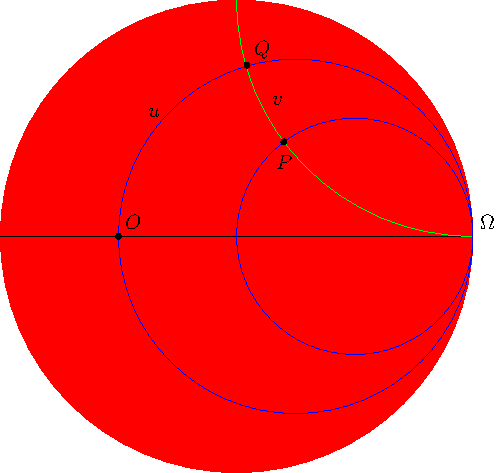
\includegraphics{images/11-horocyclebased}}
\caption{A horocycle-based coordinate system}\label{fig:horocyclecoord}
\end{figure}

We can equip it with an inner product

\[
\mathbf{a} \cdot \mathbf{b} = \begin{bmatrix} a_u & a_v \end{bmatrix} \begin{bmatrix} e^{-2v} & 0 \\ 0 & 1 \end{bmatrix} \begin{bmatrix} b_u \\ b_v \end{bmatrix}
\]

and the metrics

$$
ds^2 = e^{-2v} du^2 + dv^2
$$

Laplacian is given by\cite{Costa2001ADO}

$$
\Delta = e^{2v} \frac{\partial^2}{{\partial u}^2} + \frac{\partial^2}{{\partial v}^2} - \frac{\partial}{\partial v}
$$


\subsection{Example space II}\label{subsec:exmp2}

Giving the Poincaré disc $\mathcal{P}$ equipped with the above horocycle-based coordinate system,
we consider an assignment function $A$ defined on $\mathcal{P}$ as follows\footnote{This analytic example is provided by Le Zhang, and the geometry interpretation is given by Mingli Yuan}:

\begin{equation}
A = u e^{-v}
\end{equation}

\begin{theorem}
For the assignment $A$ in above formula, $A$ satisfy the flow equation\eqref{eq:flow}
\end{theorem}

\begin{figure}[ht]
\centering
\resizebox{0.8\textwidth}{!}{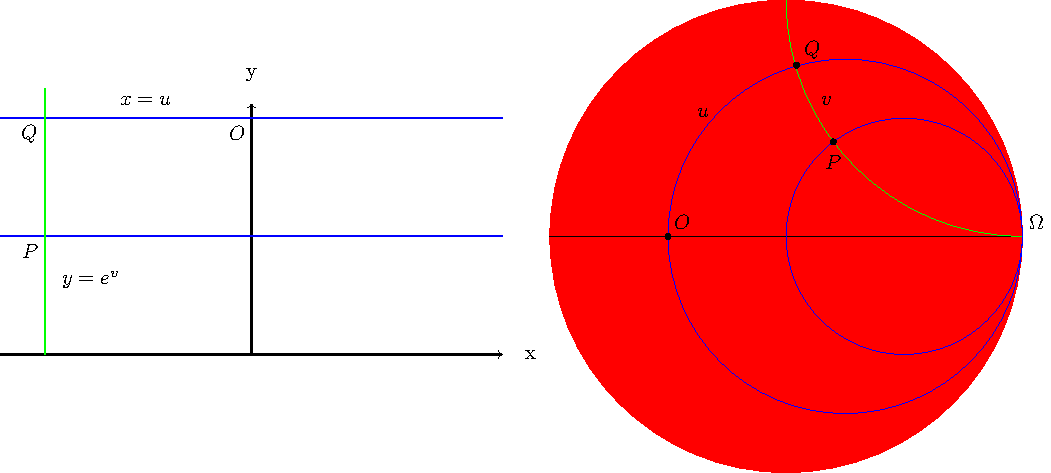
\includegraphics{images/12-proofbymapping}}
\caption{Mapping between two examples}\label{fig:mapping}
\end{figure}

\begin{proof}

If we introduce complex in the upper half plane model in last section \ref{subsec:exmp1}

$$
z = x + y i
$$

and stetup a Möbius transform between the upper half plane and current horocycle-based coordinate system:

$$
z \mapsto \frac{z-i}{z+i}
$$

This transform maps each horizontal lines in $\mathcal{H}$ into the horocycles sharing the same ideal point $\Omega = 1$ in $\mathcal{P}$,
also it maps each vertical geodesics in $\mathcal{H}$ into geodesics in $\mathcal{P}$ which are perpendicular to the above horocycles.

And rewrite the Möbius transform in the target coordinate, we get:

$$
\begin{cases}
x = u\\
y = e^v \\
\end{cases}
$$

This lead to

$$
A = -\frac{x}{y} = u e^{-v}
$$

And because of theorem \ref{thm:isometry} and Möbius transform is conformal, we can conclude that $A = u e^{-v}$ obey flow equation.

\end{proof}

We can verify $A$ is also an eigenfunction of the Laplacian
$$
\Delta A = e^{2v} \frac{\partial^2(u e^{-v})}{{\partial u}^2} + \frac{\partial^2(u e^{-v})}{{\partial v}^2} - \frac{\partial(u e^{-v})}{\partial v} = 2A
$$

From the above proof, we can see that the two assignment function $A$ arose from the same geometry setting, they are equivalent to each other.

\subsection{Generator independence}

Considering the upper half plane $\mathcal{B}$:
$$
\{\mathcal{B}: (x, y) | y > 0 \}
$$

equipped with an inner product and metrics as follows:

$$
\mathbf{a} \cdot \mathbf{b} = \begin{bmatrix} a_x & a_y \end{bmatrix} \begin{bmatrix} \frac{1}{\mu^2 y^2} & 0 \\ 0 & \frac{1}{\lambda^2 y^2} \end{bmatrix} \begin{bmatrix} b_x \\ b_y \end{bmatrix}
$$

$$
ds^2 = \frac{1}{y^2}(\frac{dx^2}{\mu^2} + \frac{dy^2}{\lambda^2})
$$

Whatever the choice of $\mu$ and $\lambda$, the assignment is given by

\begin{equation}
A = - \frac{x}{y}
\end{equation}

We can verify $A$ satisfying the flow equation\eqref{eq:flow}, and also it is generator independent.

\begin{theorem}
The above $A$ satisfying the flow equation\eqref{eq:flow}
\end{theorem}

\begin{proof}
$$
da = d(-\frac{x}{y}) = \frac{xdy - ydx}{y^2} = -\frac{dx + a dy}{y}
$$

Notice that

$$
ds = \frac{1}{y}\sqrt{\frac{dx^2}{\mu^2} + \frac{dy^2}{\lambda^2}}
$$

then

$$
\frac{da}{ds} = - \frac{dx + a dy}{y} \frac{y}{\sqrt{\frac{dx^2}{\mu^2} + \frac{dy^2}{\lambda^2}}} = \frac{dx + a dy}{\sqrt{\frac{dx^2}{\mu^2} + \frac{dy^2}{\lambda^2}}}
$$

Consider the local coordinate system given by $(-1, 0)$ and $(0, -1)$ according to the right-hand rule, we have

$$
\cos \theta = \frac{\begin{bmatrix} dx & dy \end{bmatrix} \begin{bmatrix} \frac{1}{\mu^2 y^2} & 0 \\ 0 & \frac{1}{\lambda^2 y^2} \end{bmatrix} \begin{bmatrix} -1 \\ 0 \end{bmatrix}}{\sqrt{\begin{bmatrix} dx & dy \end{bmatrix} \begin{bmatrix} \frac{1}{\mu^2 y^2} & 0 \\ 0 & \frac{1}{\lambda^2 y^2} \end{bmatrix} \begin{bmatrix} dx \\ dy \end{bmatrix}}\sqrt{\begin{bmatrix} -1 & 0 \end{bmatrix} \begin{bmatrix} \frac{1}{\mu^2 y^2} & 0 \\ 0 & \frac{1}{\lambda^2 y^2} \end{bmatrix} \begin{bmatrix} -1 \\ 0 \end{bmatrix}}}
$$

Therefore we have

$$
\cos \theta = \frac{-\frac{dx}{\mu}}{\sqrt{\frac{dx^2}{\mu^2} + \frac{dy^2}{\lambda^2}}}
$$

Similarly

$$
\sin \theta = \frac{-\frac{dy}{\lambda}}{\sqrt{\frac{dx^2}{\mu^2} + \frac{dy^2}{\lambda^2}}}
$$

Hence we have

$$
\frac{da}{ds} = \mu \cos \theta + a \lambda \sin \theta
$$

\end{proof}

tube structure of the first kind: TODO

\begin{figure}[ht]
\centering
\resizebox{1.0\textwidth}{!}{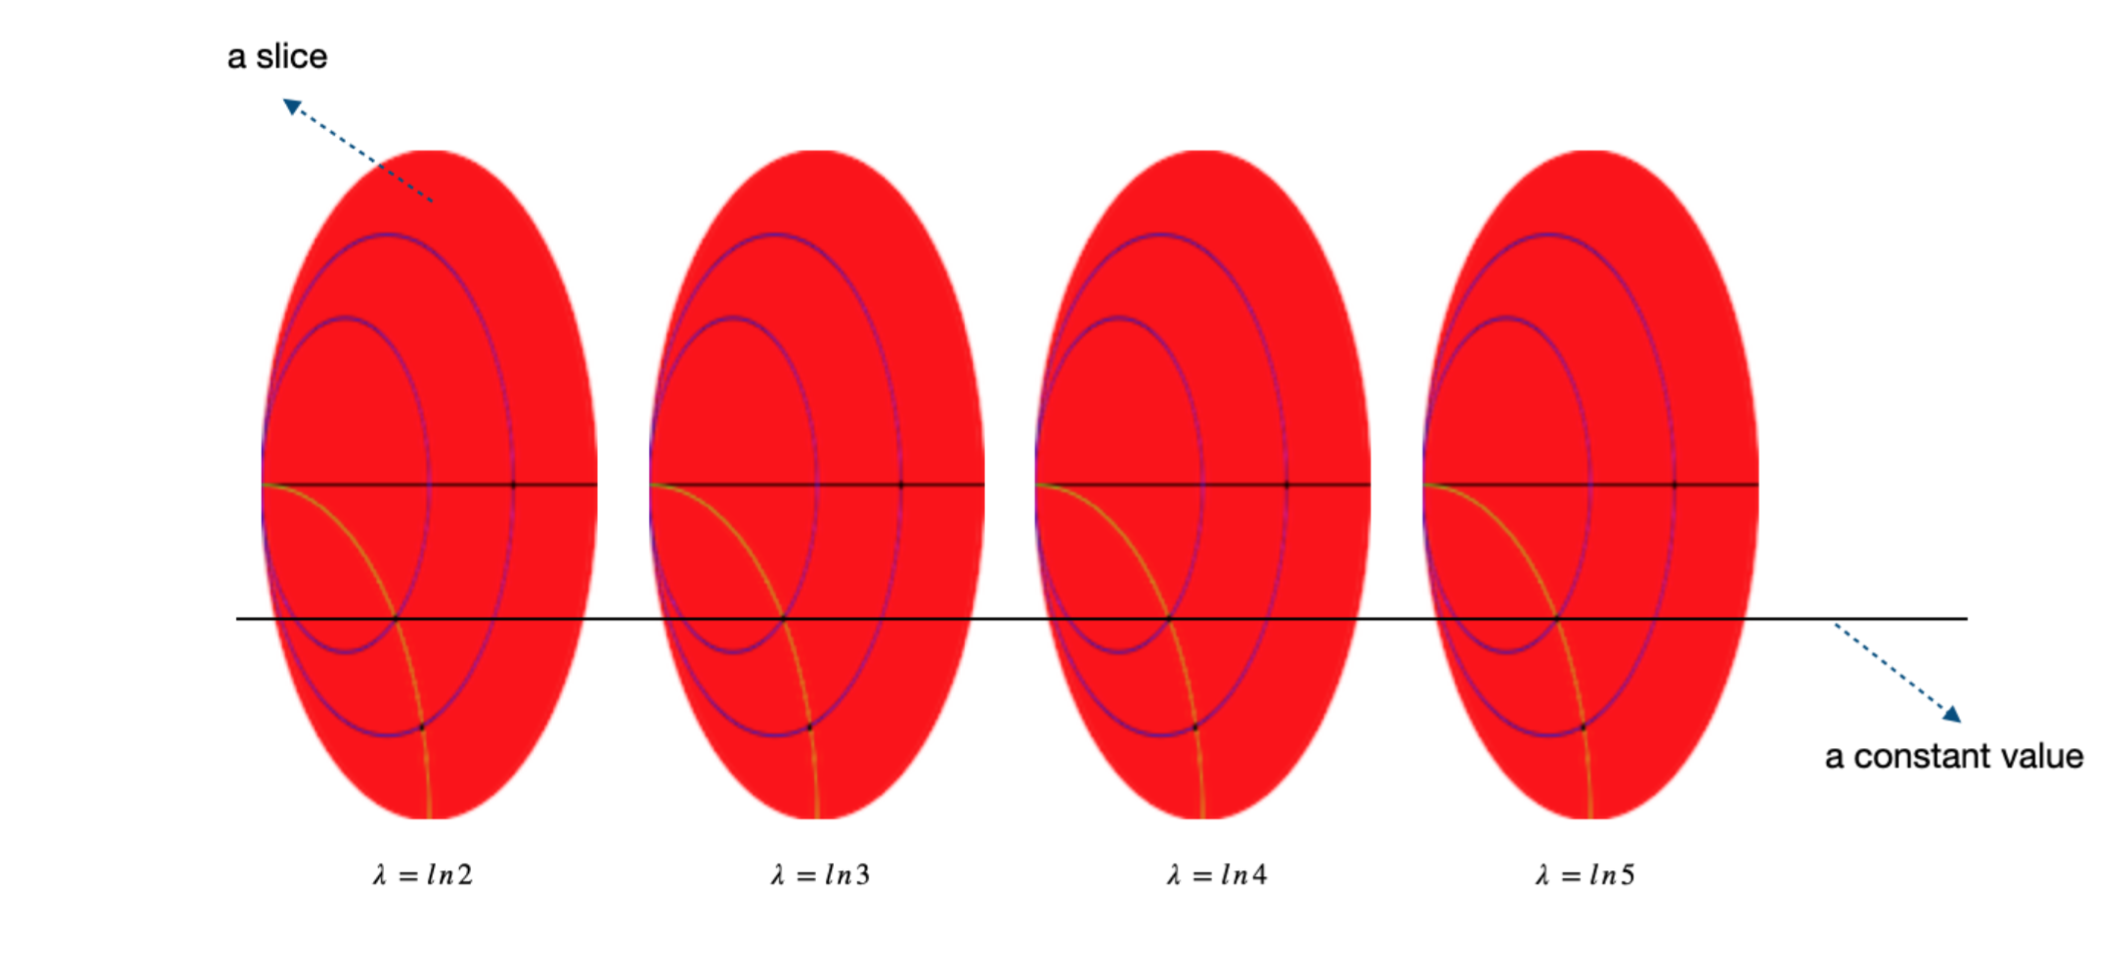
\includegraphics{images/13-tube1st.png}}
\caption{Tube structure of the first kind}\label{fig:tube1st}
\end{figure}

\subsection{Related problems}

\emph{Eigenfunction problem}: TODO.

\emph{Eigenfunction and classification problem}: TODO.

\newpage

\section{Topological arithmetic expression space}\label{sec:topology}

\subsection{The construction of the grid $G_0$}\label{sec:construction-of-grids}

To construct the grid described in subsection \ref{sec:meshgrid} and figure \ref{fig:gridex0},
we will use the number theory decomposition introduced by Victor Pambuccian in \cite{Pambuccian2016THEAO} and
Celia Schacht in \cite{Schacht2018ANOTHERAO}.

$$
n = \tau(n) \omega(n)
$$

where $\tau(n)$ is a power of 2 and $\omega(n)$ is an odd.

We can see directly from the figure \ref{fig:gridex0} that the grid is constructed by the following rules:
\begin{itemize}
\item horizantal lines (blue, additional lines) satisfying $y = 2^k, k \in \mathbb{Z}$
\item vertical lines (green, multiplicative lines) satisfying
    \begin{itemize}
        \item the value of x satisfying $x = \frac{m}{2^l}, l \in \mathbb{Z}^+, m \in \mathbb{Z}$
        \item the assignment begin from $\omega(-m)$ and increase exponentially by power 2.
    \end{itemize}
\end{itemize}

\begin{figure}[ht]
\centering
\resizebox{0.9\textwidth}{!}{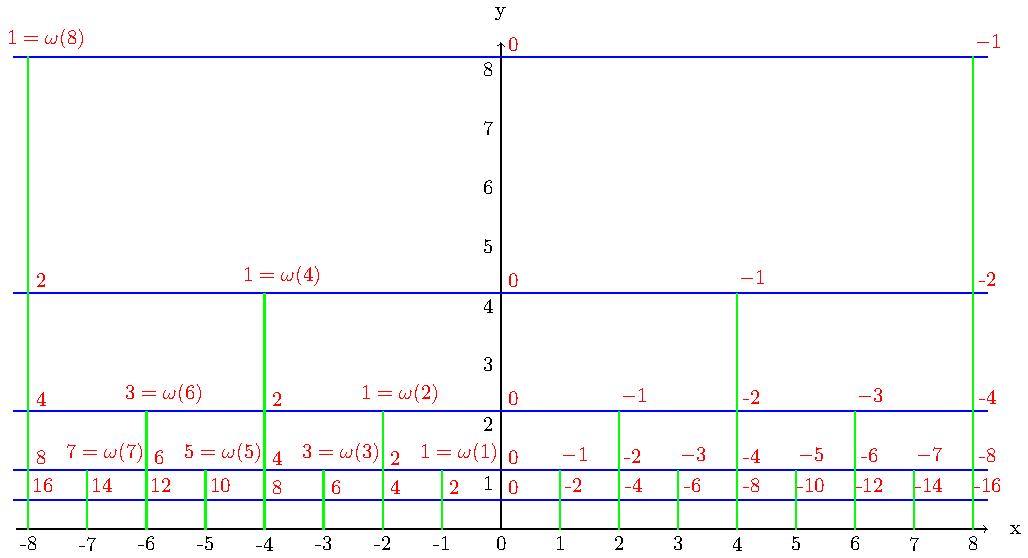
\includegraphics{images/07-grid-detail}}
\caption{$\omega$ gives the assignment at the start points of vertical lines in $G_0$}\label{fig:griddetail}
\end{figure}

The horizontal lines and the vertical lines divide the whole space into a mesh grid $G_0 = (V_0, E_0, F_0)$, where
$V_0$ is the set of crossing points, $E_0$ is the set of edges (segments in the horizontal and vertical lines,
it should be noted that only the vertical lines are geodesics, while the horizontal lines are horocycles) connecting
the crossing points, and $F_0$ is the set of cut cells. This mesh grid is generated by the additional generator $1$ and
the multiplicative generator $2$, and $V_0$, $E_0$, and $F_0$ are all countable sets.

We illustrate the construction schema of $G_0$ in Figure \ref{fig:gridschema}.

\begin{figure}[ht]
\centering
\resizebox{0.9\textwidth}{!}{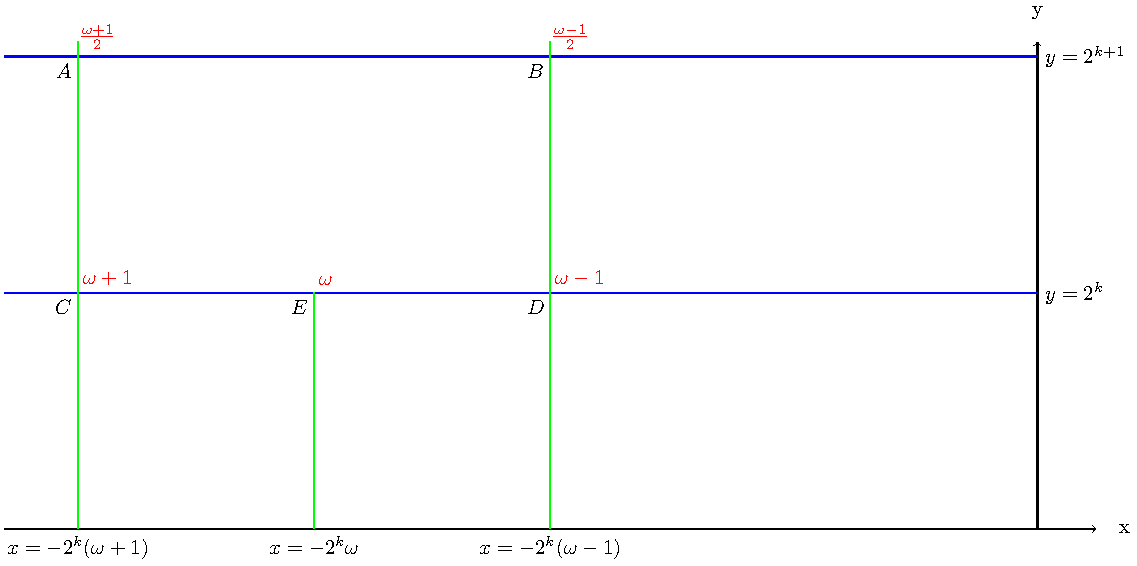
\includegraphics{images/08-grid-schema}}
\caption{the construction schema of $G_0$}\label{fig:gridschema}
\end{figure}

We notice that $G_0$ is very regular, in fact, all edges are equidistant.

\begin{lemma}\label{lem:regular}
All edges in $G_0$ are equidistant.
\end{lemma}

\begin{proof}
Following the construction schema in Figure \ref{fig:gridschema}, we can calculate the length of segments are all equidistant.

Length of $AC$ and $BD$:

$$
\int ds = \int\limits_{2^{k}}^{2^{k+1}} \frac{1}{y \ln 2} dy = \frac{1}{\ln 2} \left( \ln 2^{k+1} - \ln 2^k \right) = 1
$$

Length of $AB$:

$$
\int ds = \int\limits_{-2^k(\omega + 1)}^{-2^k(\omega - 1)} \frac{1}{2^{k+1}} dx = \frac{1}{2^{k+1}} \left( 2^{k + 1} \right) = 1
$$

Length of $CE$:

$$
\int ds = \int\limits_{-2^k(\omega + 1)}^{-2^k \omega} \frac{1}{2^k} dx = \frac{1}{2^k} \left( 2^k \right) = 1
$$

Length of $ED$:

$$
\int ds = \int\limits_{-2^k \omega}^{-2^k(\omega - 1)} \frac{1}{2^k} dx = \frac{1}{2^k} \left( 2^k \right) = 1
$$
\end{proof}

\subsection{The construction of the grid $G_1$}\label{sec:construction-of-grids}

We can similarly construct the grid $G_1$ using the additional generator $\frac{1}{2}$ and the multiplicative generator
$\sqrt{2}$, the grid $G_2$ using the additional generator $\frac{1}{4}$ and the multiplicative generator $\sqrt[4]{2}$,
and so on. And each time the cell of the mesh grid is divided into smaller cells and the end points of the vertical lines
move upward.

\begin{figure}[ht]
\centering
\resizebox{0.9\textwidth}{!}{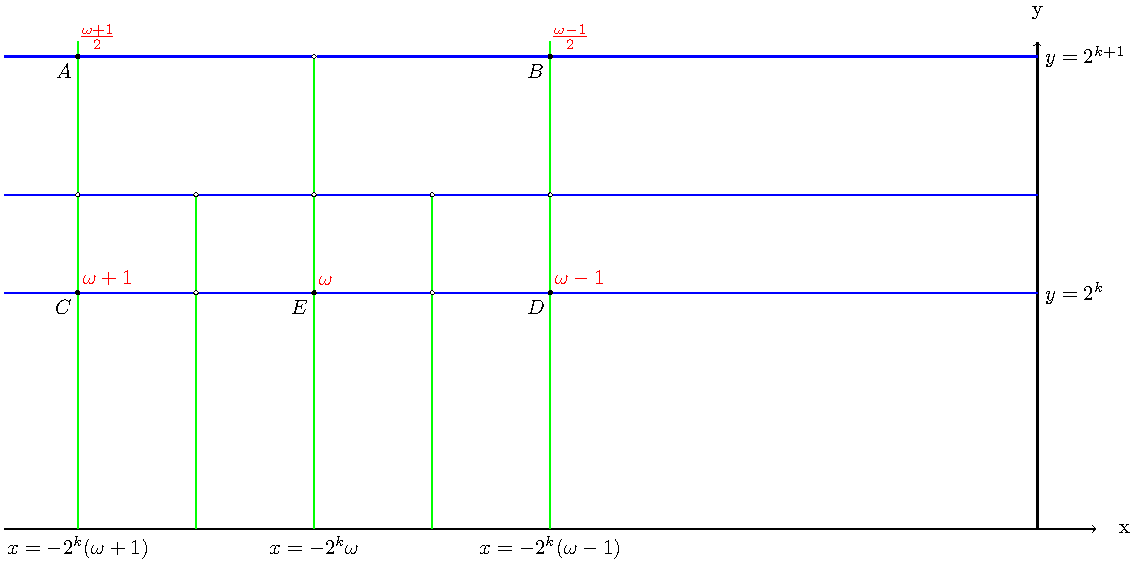
\includegraphics{images/09-grid-schema-g1}}
\caption{the construction schema of $G_1$}\label{fig:gridschemag1}
\end{figure}

\subsection{The construction of the grid $G_2$}\label{sec:construction-of-grids}


\subsection{The grid mesh is dense}\label{sec:construction-of-grids}

It is easy to see that there is a chain of inclusion relations:
$$
V_0 \subset V_1 \subset V_2 \subset \cdots V_i \subset \cdots
$$

Suppose $V = \bigcup_{i=1}^{\infty} V_i$, we have below lemma

\begin{lemma}
$V$ is a countable dense set.
\end{lemma}

\begin{proof}
Because $V_i$ is countable, and the union is over a countable index set, so $V$ is countable.

We can prove it is dense by contradiction. Suppose $V$ is not a dense set. Then there is a point $p$ in the space
neither belongs to $V$ nor is a limit point of $V$.

TODO...

\end{proof}

\subsection{Completeness and topology}\label{sec:topdef}

\subsection{As a special integral}\label{sec:integral}

\newpage

\section{On order-4 apeirogonal tiling}\label{sec:tiling}

\subsection{Construction of order-4 apeirogonal tiling}\label{sec:tiling}

\newpage

\section{New perspectives and methods}\label{sec:function}

\subsection{On integral theory}\label{sec:integral}

\subsection{On representation of function}\label{sec:function}

\subsection{Questions related with complexity?}\label{sec:complexity}

\newpage

\section{A glossary of unsolved problems}\label{sec:problems}

\subsection{Foundation questions}\label{sec:foundation}

\subsection{Classification problem}\label{sec:donaghey}

\subsection{Eigenfunction problem}\label{sec:eigenfunction}

\subsubsection{The second kind of arithmetic expression space}\label{sec:secondkind}

\subsubsection{The third kind of arithmetic expression space}\label{sec:thirdkind}

\subsection{Harmonic problem}\label{sec:harmonic}

\subsection{Tube structure}\label{sec:tube}

\subsection{Singular points and divergent series}\label{sec:singularity}

\subsection{Function and a new caculus?}\label{sec:caculus}

\subsection{Category of function theories?}\label{sec:function}

\subsection{Geometrilization of computation}\label{sec:computation}

\subsection{Geometrilization of logic}\label{sec:logic}
\subsubsection{irrationality of $\sqrt{17}$}

\bibliographystyle{plain}
\bibliography{aeg-paper.bib}

\appendix

\section{A direct formal solution of the flow equation}\label{sec:directformalsolution}

We can also get a direct formal solution of the flow equation (\eqref{eq:flow}) step by step:

$$
    \frac{da}{\mu \cos \theta + a \lambda \sin \theta} = ds
$$

$$
    \frac{1}{\lambda \sin \theta} \frac{d(\mu \cos \theta + a \lambda \sin \theta)}{\mu \cos \theta + a \lambda \sin \theta} = ds
$$

$$
    \frac{1}{\lambda \sin \theta} ln(\mu \cos \theta + a \lambda \sin \theta) = s + C
$$

$$
    \mu \cos \theta + a \lambda \sin \theta = e^{\lambda s \sin \theta} e^{C \lambda \sin \theta}
$$

Considering the initial condition
$$
    \mu \cos \theta + a_0 \lambda \sin \theta = e^{C \lambda \sin \theta}
$$

We have
$$
    \mu \cos \theta + a \lambda \sin \theta = e^{\lambda s \sin \theta} (\mu \cos \theta + a_0 \lambda \sin \theta)
$$

$$
   a = \frac{\mu \cos \theta + a_0 \lambda \sin \theta}{\lambda \sin \theta} e^{\lambda s \sin \theta} - \frac{\mu}{\lambda}\cot \theta
$$

$$
   a = (a_0 + \frac{\mu}{\lambda} \cot \theta) e^{\lambda s \sin \theta} - \frac{\mu}{\lambda} \cot \theta
$$

\begin{equation}
   a =  a_0 e^{\lambda s \sin \theta} + \frac{\mu}{\lambda} (e^{\lambda s \sin \theta} - 1) \cot \theta
\end{equation}

\begin{equation}\label{eq:directformalsolution}
   a =  a_0 e^{\lambda s \sin \theta} + \frac{\mu}{\lambda} (e^{\lambda s \sin \theta} - 1) \cot \theta
\end{equation}

\section{Conformance between infinitesimal generating process and discrete mesh grid}\label{sec:conformance}

In order to verify the conformance, we expand the formula \eqref{eq:directformalsolution} in the following way:

\begin{equation}
   a =  a_0 e^{\lambda s \sin \theta} + \frac{\mu}{\lambda} [1 + \lambda s \sin \theta + \frac{1}{2!} (\lambda s \sin \theta)^2  + \frac{1}{3!} (\lambda s \sin \theta)^3 + \cdots - 1] \cot \theta
\end{equation}

\begin{equation}
   a = a_0 e^{\lambda s \sin \theta} + \mu s \cos \theta + \frac{\mu}{\lambda} \sin \theta \cos \theta (\frac{\lambda^2s^2}{2!} + \frac{\lambda^3s^3}{3!} \sin \theta + \frac{\lambda^4s^4}{4!} \sin^2 \theta + \cdots)
\end{equation}

\begin{equation}
   a = a_0 e^{\lambda s \sin \theta} + \mu s \cos \theta + \frac{\mu}{2\lambda} \sin 2\theta (\frac{\lambda^2s^2}{2!} + \frac{\lambda^3s^3}{3!} \sin \theta + \frac{\lambda^4s^4}{4!} \sin^2 \theta + \cdots)
\end{equation}

\begin{equation}
   a = a_0 e^{\lambda s \sin \theta} + \mu s \cos \theta + \frac{\mu}{2\lambda} \Psi(s) \sin 2\theta
\end{equation}

When $\theta = \frac{k \pi}{2}, k = 0, 1, 2, 3\cdots, s = 0, 1, 2, 3\cdots$, we have

\begin{equation}
    a = a_0 e^{\lambda s \sin \theta} + \mu s \cos \theta
\end{equation}

Especially, we have

\begin{equation}
    a = a_0 + \mu s, s = 0, 1, 2, 3\cdots, k = 0, 1, 2, 3\cdots, \theta = 2k\pi
\end{equation}

\begin{equation}
    a = x_0e^{\lambda s}, s = 0, 1, 2, 3\cdots, k = 0, 1, 2, 3\cdots, \theta = 2k\pi + \frac{\pi}{2}
\end{equation}

\begin{equation}
    a = a_0 - \mu s, s = 0, 1, 2, 3\cdots, k = 0, 1, 2, 3\cdots, \theta = 2k\pi + \pi
\end{equation}

\begin{equation}
    a = a_0 e^{- \lambda s}, s = 0, 1, 2, 3\cdots, k = 0, 1, 2, 3\cdots, \theta = 2k\pi + \frac{3 \pi}{2}
\end{equation}

which gives the conformance.

\section{Arithmetic expression, combinators and transformation over trees}\label{sec:expressions}

\subsection{LISP and combinators}\label{sec:donaghey}

\subsection{Applicative and concatenative}\label{sec:donaghey}

\subsection{Donaghey transformation}\label{sec:donaghey}

\newpage


\end{document}
